\documentclass[convert={imagemagick, density=1024}]{standalone}
\usepackage{tikz}
\begin{document}
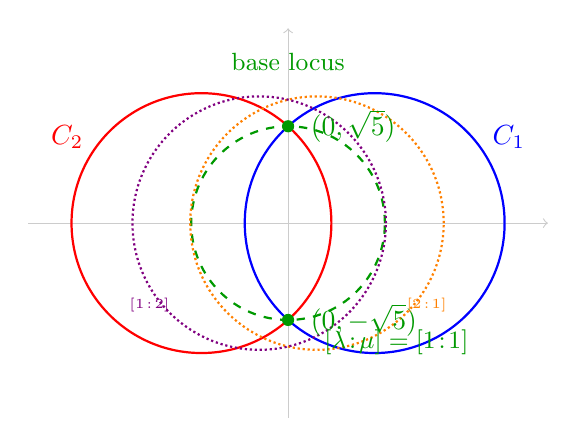
\begin{tikzpicture}[scale=0.55]
  % axes
  \draw[gray!40, ->] (-6,0) -- (6,0);
  \draw[gray!40, ->] (0,-4.5) -- (0,4.5);

  % C1: center (2,0), radius 3
  \draw[blue, thick] (2,0) circle (3);
  % C2: center (-2,0), radius 3
  \draw[red, thick] (-2,0) circle (3);

  % Pencil elements (lambda:mu)
  % [1:1] -> center (0,0), radius sqrt(5) ~ 2.236
  \draw[green!60!black, thick, dashed] (0,0) circle (2.236);

  % [2:1]: center = (2*2*1-2*1*2)/(2+1)... let's compute:
  % F1 + 2F2: 3(x^2+y^2-5) + 4*2x = ... actually let me just pick nice ones
  % [3:1]: (x-6/4)^2 + y^2 = 9 - 36/16 + ... let me just pick [2:-1] etc.
  % Simpler: [1:2] -> center (-2/3,0), radius = sqrt(9 - 4/9) = sqrt(77/9) ~ 2.93
  % [2:1] -> center (2/3,0), radius ~ 2.93
  \draw[orange, thick, densely dotted] (0.667,0) circle (2.926);
  \draw[violet, thick, densely dotted] (-0.667,0) circle (2.926);

  % intersection points
  \fill[green!60!black] (0, 2.236) circle (4pt);
  \fill[green!60!black] (0,-2.236) circle (4pt);

  % labels
  \node[blue, above right] at (4.5, 1.5) {$C_1$};
  \node[red, above left] at (-4.5, 1.5) {$C_2$};
  \node[green!60!black, right] at (0.3, 2.236) {$(0, \sqrt{5})$};
  \node[green!60!black, right] at (0.3,-2.236) {$(0, -\sqrt{5})$};

  % base locus label
  \node[green!60!black, above] at (0, 3.3) {\small base locus};

  % pencil element labels
  \node[green!60!black, below] at (2.5,-2.236) {\small $[\lambda\!:\!\mu]=[1\!:\!1]$};
  \node[orange, below] at (3.2,-1.5) {\tiny $[2\!:\!1]$};
  \node[violet, below] at (-3.2,-1.5) {\tiny $[1\!:\!2]$};
\end{tikzpicture}
\end{document}
